%Vytvoril: Maroš Orsak
%xorsak02
%2017

\documentclass{beamer}
\mode<presentation> {
\usetheme{Warsaw}
\setbeamercovered{transparent}
}
\usecolortheme{whale}

\usepackage[export]{adjustbox} % pouzitie kvoli picture position
\usepackage[utf8]{inputenc}
\usepackage[czech]{babel}
\usepackage{times}
\usepackage{graphics}
\usepackage{amsmath, amsthm, amssymb}

\title{Typografia}
\author{\texorpdfstring{Maroš Orsák \ \newline\url{xorsak02@stud.fit.vutbr.cz}}{Author}}
\institute{Vysoké učenie technické v~Brně \\Fakulta informačných technológií}
\date{1. 5. 2017}

\addto\captionsczech{\renewcommand{\figurename}{Obrázok}}

\begin{document}
\begin{frame}
\titlepage
\end{frame}

\begin{frame}
\frametitle{Typografia}
\begin{itemize}
\item{je umělecko-technický obor, který se zabývá tiskovým písmem}
\item{dělí se na:}
\begin{itemize}
\item{mikrotypografii}
\item{makrotypografii}
\end{itemize}
\end{itemize}
\textbf{Mikrotypografii}
\begin{itemize}
\item{se zabývá uměleckou tvorbou písma}
\end{itemize}
\textbf{Makrotypografii}
\begin{itemize}
\item{se zabývá umístěním písma na stránku proporcemi titulků , textu , ilustrací \dots}
\item{v češtině se tradičně nazývá grafická úprava}
\end{itemize}
\end{frame}
%2%%%%%%%%%%%%%%%%%%%%%%%%
\begin{frame}
\frametitle{Dejiny}
\begin{itemize}
\item{začínají na přelomu středověku a novověku kolem poloviny 16. století}
\item{nejčastěji se za vynálezce označuje Johannes Gutenberg, který v Mohuči v roce 1448 uvedl do provozu knihtisk z dřevěných matric}
\item{v českých zemích se etablovaly knihtiskárny velmi časně, nejprve roku 1468 tiskem Trojánské kroniky v Plzni a v dalším desetiletí v Praze.}
\item{v roce 1465 Konrad Sweynheim a Arnold Pannartz vydali Ciceronův spis De oratore antikvou (Antiqua, anglicky Roman)}
\end{itemize}
\end{frame}
%3%%%%%%%%%%%%%%%%%%%%%%%
\begin{frame}
\frametitle{Dejiny}
\begin{itemize}
\item{novým obdobím zásadního rozvoje typografie bylo baroko (anglicky Transitional, 1722–1763), de facto tedy rokoko.}
\end{itemize}
\textbf{Barok}
\begin{itemize}
\item{vyznačuje se v písmu větším kontrastem mezi širokými dříky písmen a úzkými liniemi a důsledným oddělováním titulků, odstavců \dots}
\end{itemize}
\textbf{Klasicizmus}
\begin{itemize}
\item{pod vlivem objemných tisků encyklopedií ještě zvýšil technický charakter písma a kontrast mezi tenkými a tlustými liniemi}
\item{písmo je užší a sklon přímější}
\end{itemize}
\end{frame}
%4%%%%%%%%%%%%%%%%%%%%%%%%%
\begin{frame}
\frametitle{Dejiny}
\textbf{19.století}
\begin{itemize}
\item{Obnova estetické kvality typografie}
\end{itemize}
\textbf{20.století}
\begin{itemize}
\item{zavedení digitálního tisku}
\item{dosavadní typy krásného písma se zprvu drasticky redukovaly podle omezených možností výstupní techniky}
\item{dalším technickým pokrokem se v posledních letech postupně vrací estetické normy typografie, ovšem nemají již masové měřítko tisku na papíře, nýbrž pronikají více do elektronických médií}
\end{itemize}
\end{frame}
%5%%%%%%%%%%%%%%%%%%%%%%%%%
\begin{frame}
\frametitle{Proslulí světoví typografové}
\textbf{Nicolas Jenson (1420-1480)}
\begin{itemize}
\item{byl původem Francouz, tiskař v Benátkách}
\item{ Edicí Ciceronových Epistolae ad Brutum (1470) obnovil antikvu do dnešní podoby}
\end{itemize}
\textbf{Frederic William Goudy (1865–1947)}
\begin{itemize}
\item{byl americký tiskař}
\item{jeho nejslavnějším písmem je Goudy Old Style}
\end{itemize}
\textbf{William Addison Dwiggins (1880–1956)}
\begin{itemize}
\item{byl žákem Goudyho} 
\item {Vytvořil pro Linotype tato písma:} 
\begin{itemize}
\item{Caledonia}
\item{Electra}
\item{Eldorado}
\item{Metro}
\end{itemize}
\end{itemize}
\end{frame}
%Frederic Wiliam Goudy%%%%%%%%%%%%%%%%%%
\begin{frame}
\frametitle{Proslulí světoví typografové}
\begin{figure}[Htbp]
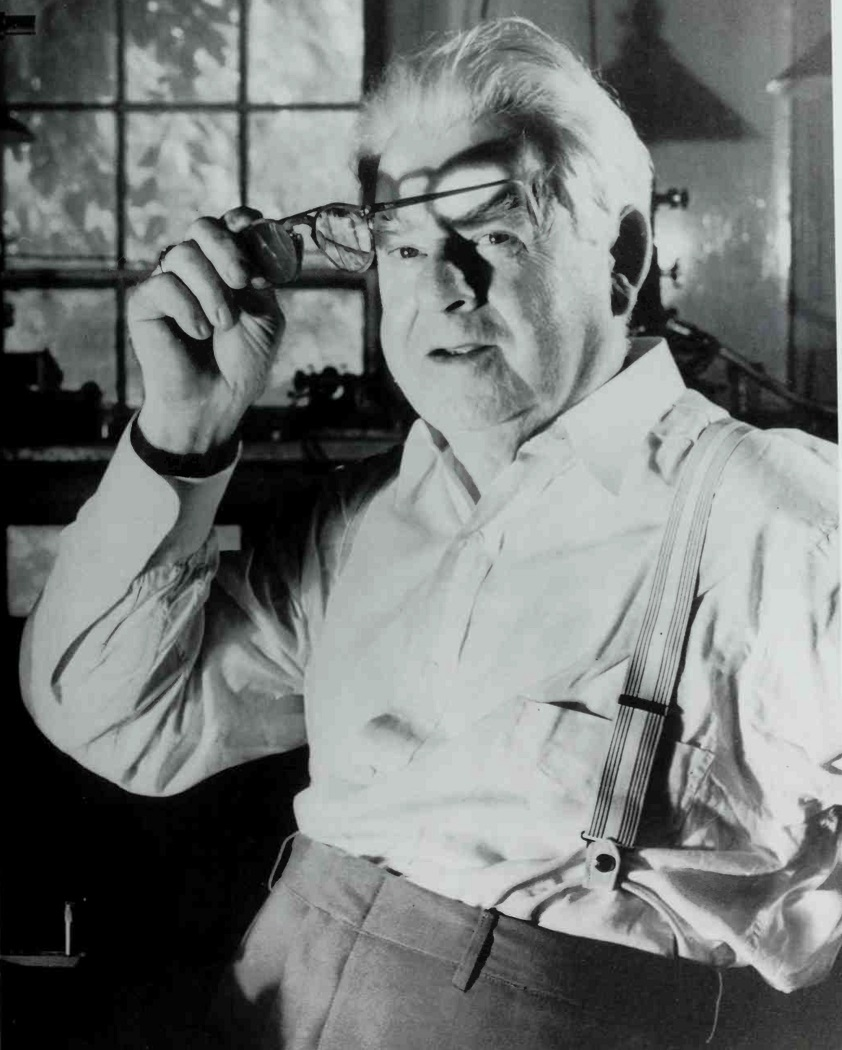
\includegraphics[scale = 0.18]{FredericGoudy.jpg}
\caption{Frederic Wiliam Goudy }
\end{figure}
\end{frame}
%Wiliam Addison Dwiggins%%%%%%%%%%%%%%%%%%
\begin{frame}
\frametitle{Proslulí světoví typografové}
\begin{figure}[Htbp]
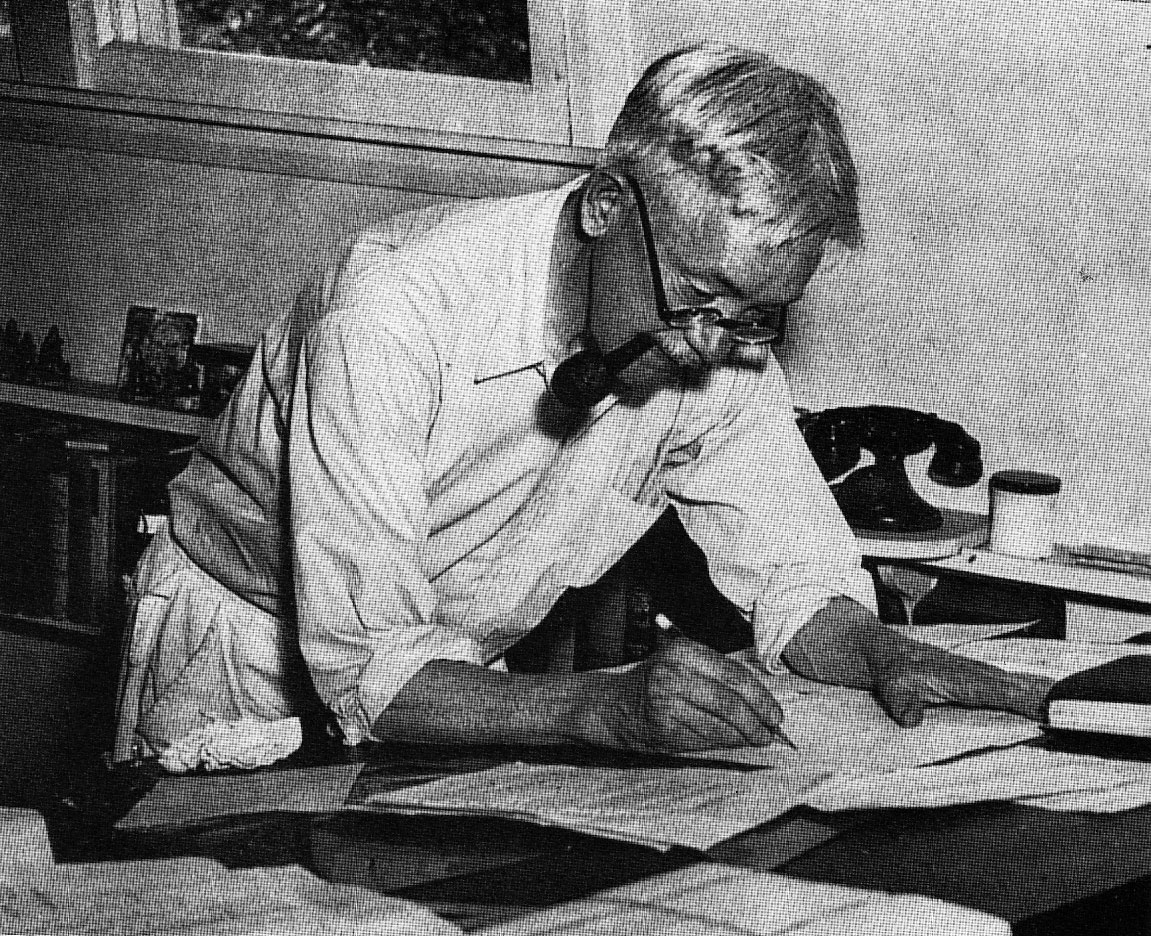
\includegraphics[scale = 0.20]{William-Addison-Dwiggins.jpg}
\caption{William Addison Dwiggins}
\end{figure}
\end{frame}

%6%%%%%%%%%%%%%%%%%%%%%%%%
\begin{frame}
\frametitle{Použitá literatúra}
\begin{itemize}
\item{Jiří Rybička: Latex pro začatečníky}
\item{\texttt{https://cs.wikipedia.org/wiki/Typografie}}

\end{itemize}
\end{frame}

\end{document}


